\documentclass{article}

\title{Nostoi\\ \normalsize a functionality that lets you \emph{go home}}

\usepackage{graphicx, amsmath}
\usepackage{fourier}
\begin{document}
\maketitle
Point a finger on the world map choosing your starting city $a$:
\begin{center}
  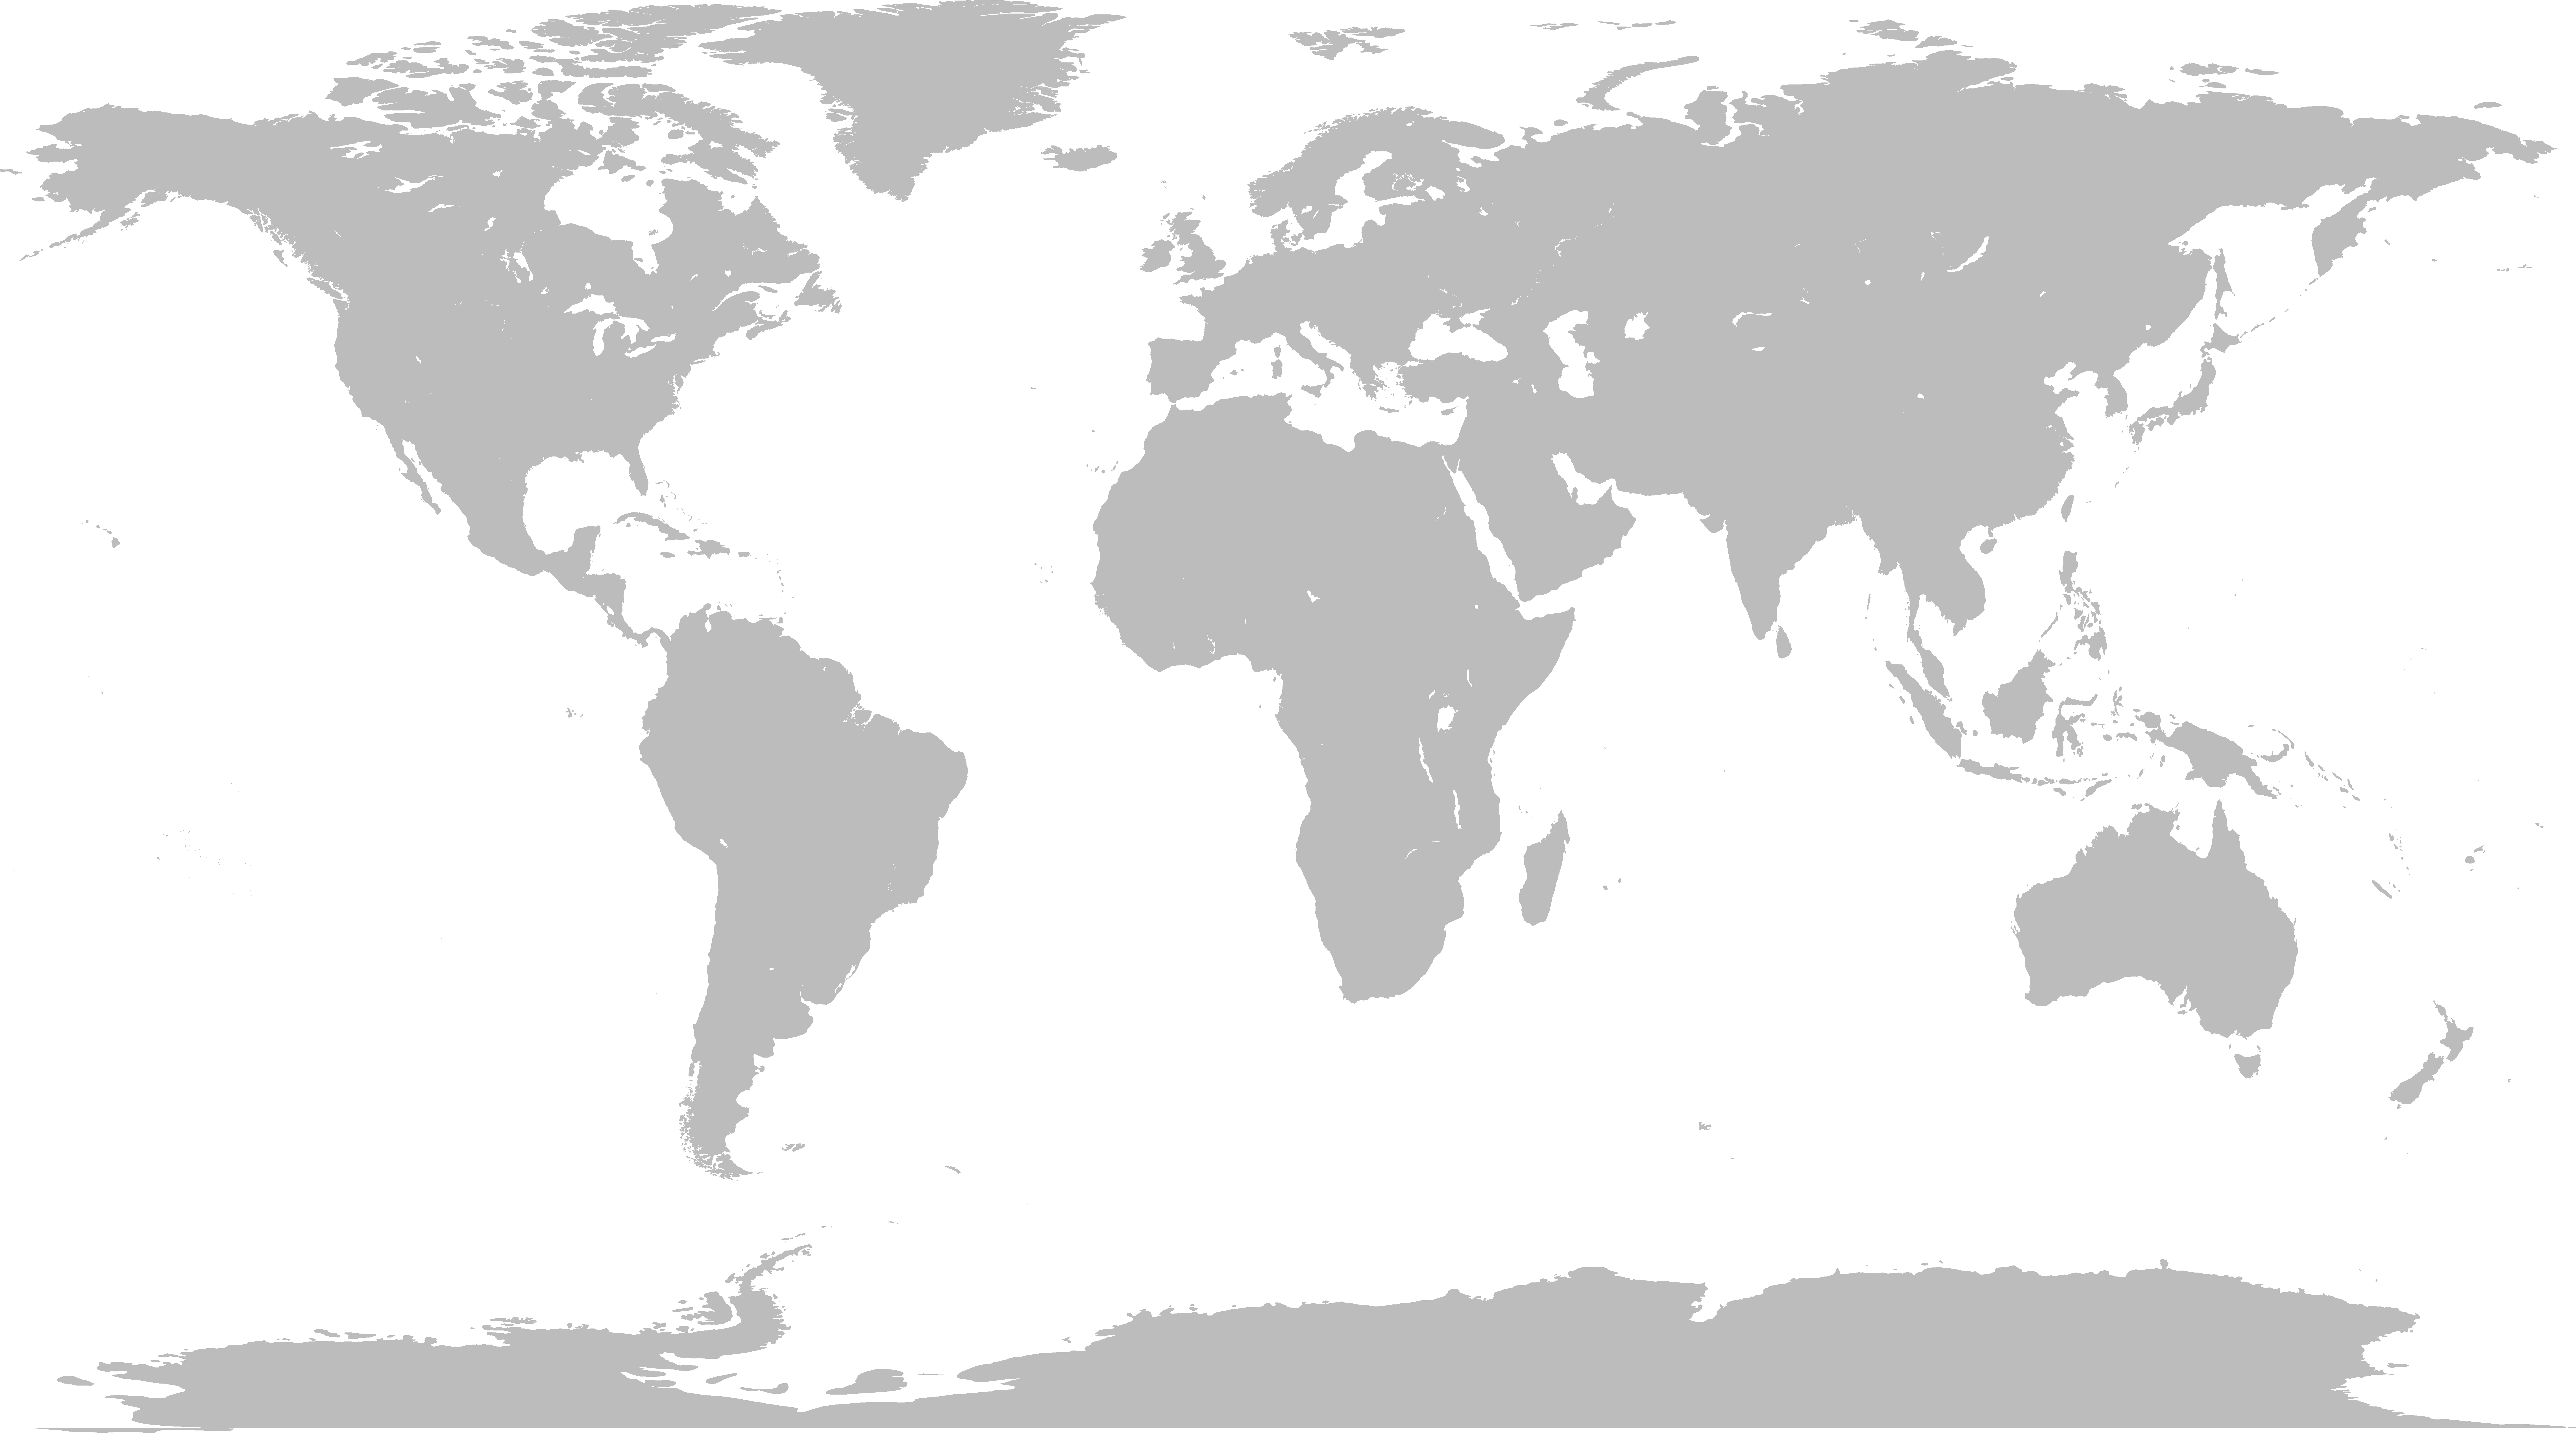
\includegraphics[width=.9\textwidth]{world}
\end{center}
Construct the \emph{isotherms} with respect to a cost function
\[
  \textsf{mana}(a,b) = \mu(a,b) + \Delta d(a,b) + \Delta t(a,b) + f(a,b) %+ \varrho(a,b)
\] where
\begin{itemize}
  \item $\mu$ is the expense of the trip from $a$ to $b$;
  \item $\Delta d$ is the (orthodromic) distance $\widearc{ab}$;
  \item $\Delta t$ is the minimal flight time from $a$ to $b$;
  \item $f$ accounts for the frequency of flights in the range 00:00 - 23:59;
\end{itemize}
A further meaningful quantity associated to the trajectory $\widearc{ab}$ is the \emph{symmetry} $\varrho(a,b)$; it measures how symmetric the ``distance'' between $a,b$ is according to (something similar to) a sigmoid function of the mana.
\end{document}